\chapter{The Transit Monitoring in the South project}\label{chap:tramos}

The Transit Monitoring in the South (TraMoS) project started in 2008 aiming to perform photometric follow-up of transiting exoplanets using telescopes located in Chile.  Through photometric monitoring of transiting events, important information of the planetary system can be obtained, such as the planetary radius, inclination of the orbit, precise planetary mass, among others. Moreover, this kind of analysis allows the detection of variability in the transit's parameters (TPV), if several epochs of the transit event are included. The TraMoS project aims, on the one hand, to refine the physical and orbital parameters of selected exoplanets systems through photometric follow-up and, on the other hand, to search variations in that parameters that could suggest the presence of additional bodies in the system. 

To date, almost 400 transit events have been observed of 144 transiting exoplanets (see Figure \ref{tramos}). The bulk of the targets in the TraMoS project are hot Jupiters due to its short orbital period and large transit depth. Several facilities were used to perform the photometric follow-up such as the VLT of European Southern Observatory, the SMARTS 0.9 m and 1 m at Cerro Tololo Inter-American Observatory, the Danish 1.54 m at La Silla Observatory, SWOPE and Du Pont telescopes at Las Campanas Observatory and SOAR telescope at Cerro Pachón Observatory, among others. The diameter size of the used telescopes ranges from 0.6 meters to 8 meters. However, in the last stage of the TraMoS project, we built the team expertise using 1 meter-class telescopes, for example in the Danish, SWOPE and SMARTS.

\begin{figure}
\centering
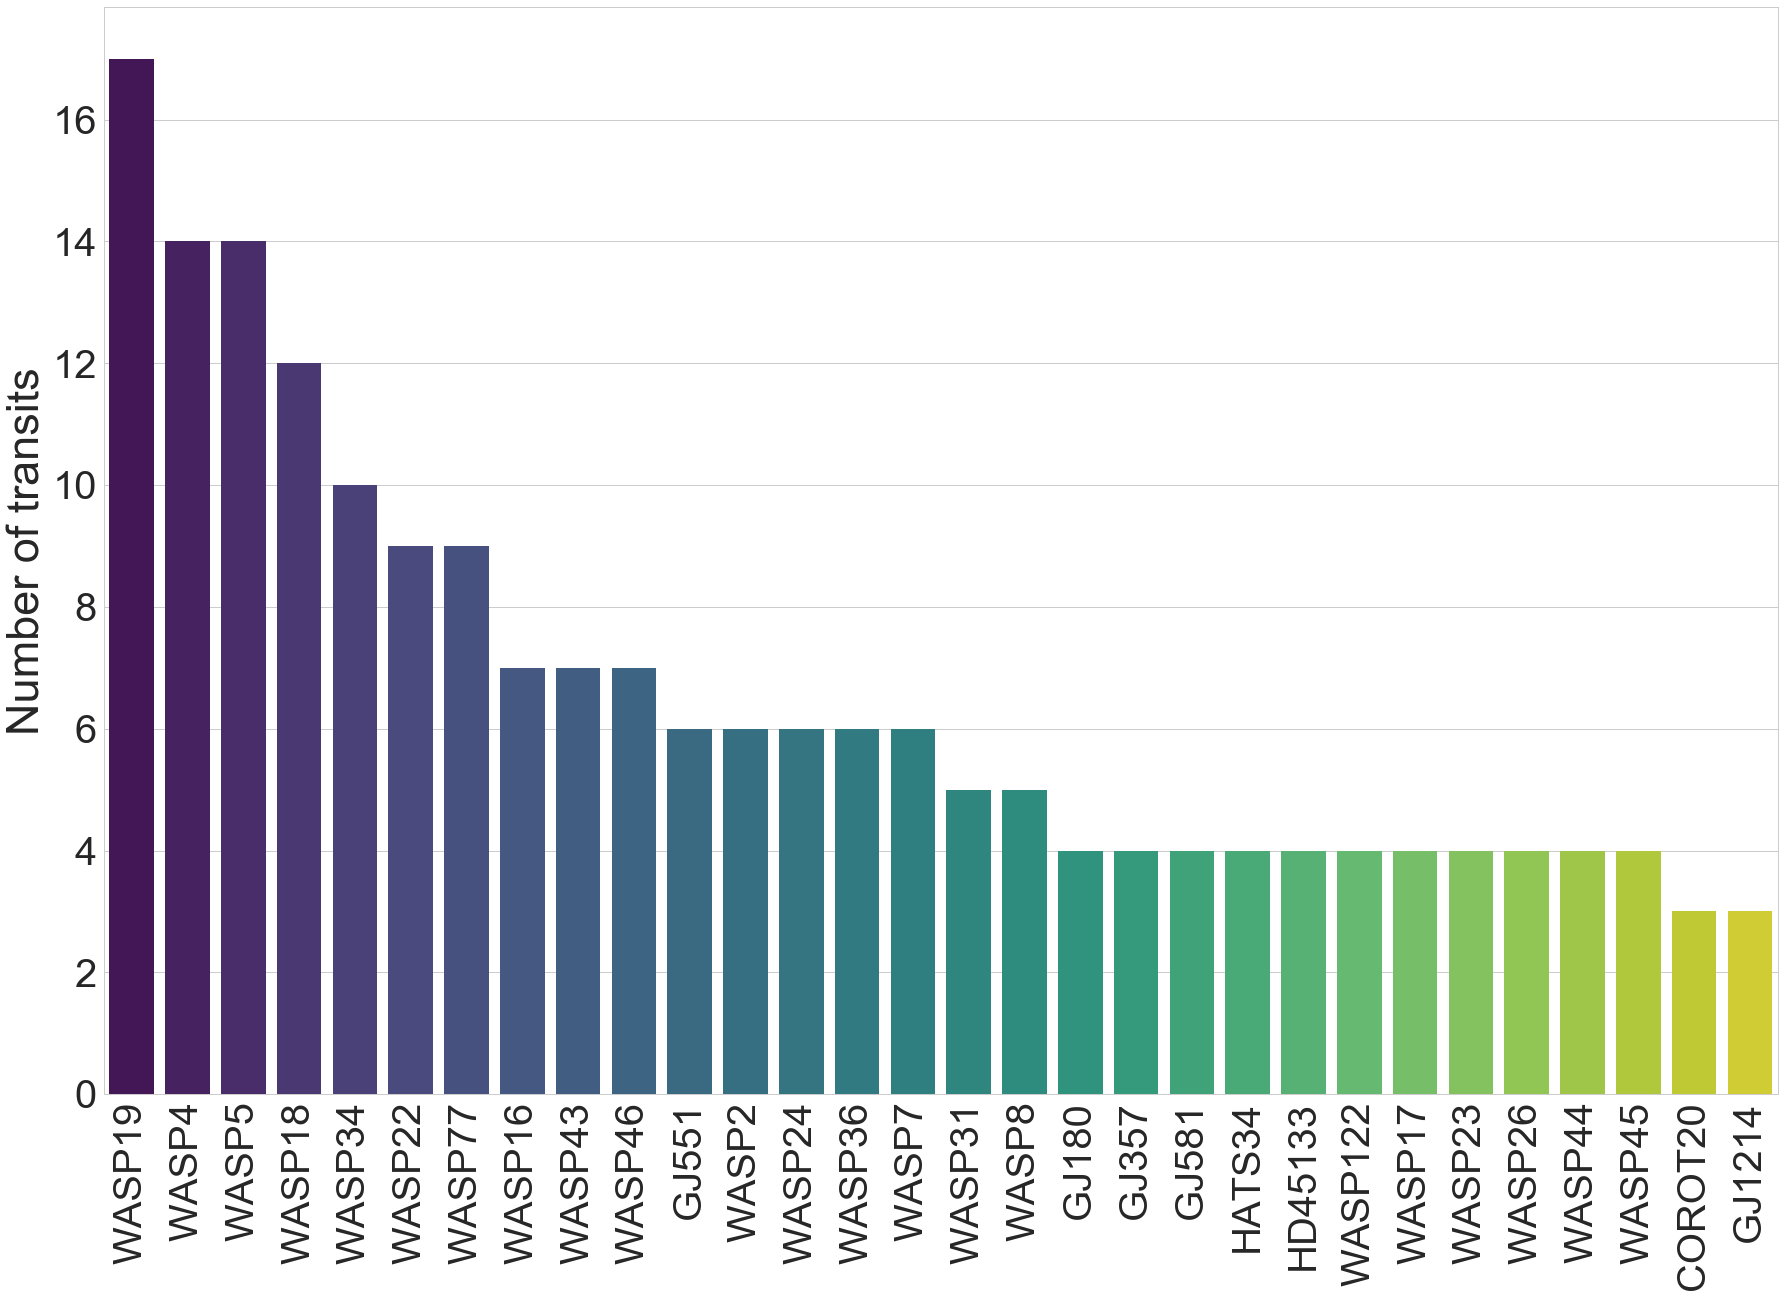
\includegraphics[width=1.0\columnwidth]{imagenes/tramos.png}
\caption{Histogram of the 30 transiting exoplanets with the largest amount of observations within the TraMoS project. The exoplanets WASP-4b and WASP5-b were presented in \cite{Hoyer2012} and \cite{Hoyer2013}. The results from the analysis of WASP-18b, WASP-19b and WASP77-Ab are in Cortés-Zuleta et al. 2019 (submitted, see Chapter \ref{chap:paper} for further details). In any of those systems a significant TTV signal was detected.}
\label{tramos}
\end{figure}


The first studies within the TraMoS project were conducted by Sergio Hoyer, former PhD student of Professor Patricio Rojo. In summary, a possible orbital decay of WASP-43b \citep{Hoyer2016b} and OGLE-TR-113b \citep{Hoyer2016} was ruled out, and no significant TTV signal was detected in WASP-4b \citep{Hoyer2012} and WASP-5b \citep{Hoyer2013}.

\section{Transiting Exoplanets}
The Transit method is today the most successful technique to discover extrasolar planets (see Fig.~\ref{amount_exoplanet}). The Kepler mission was launched in 2009 and during its almost nine years of provided thousands of discoveries due to this method.

\begin{figure}[H]
\centering
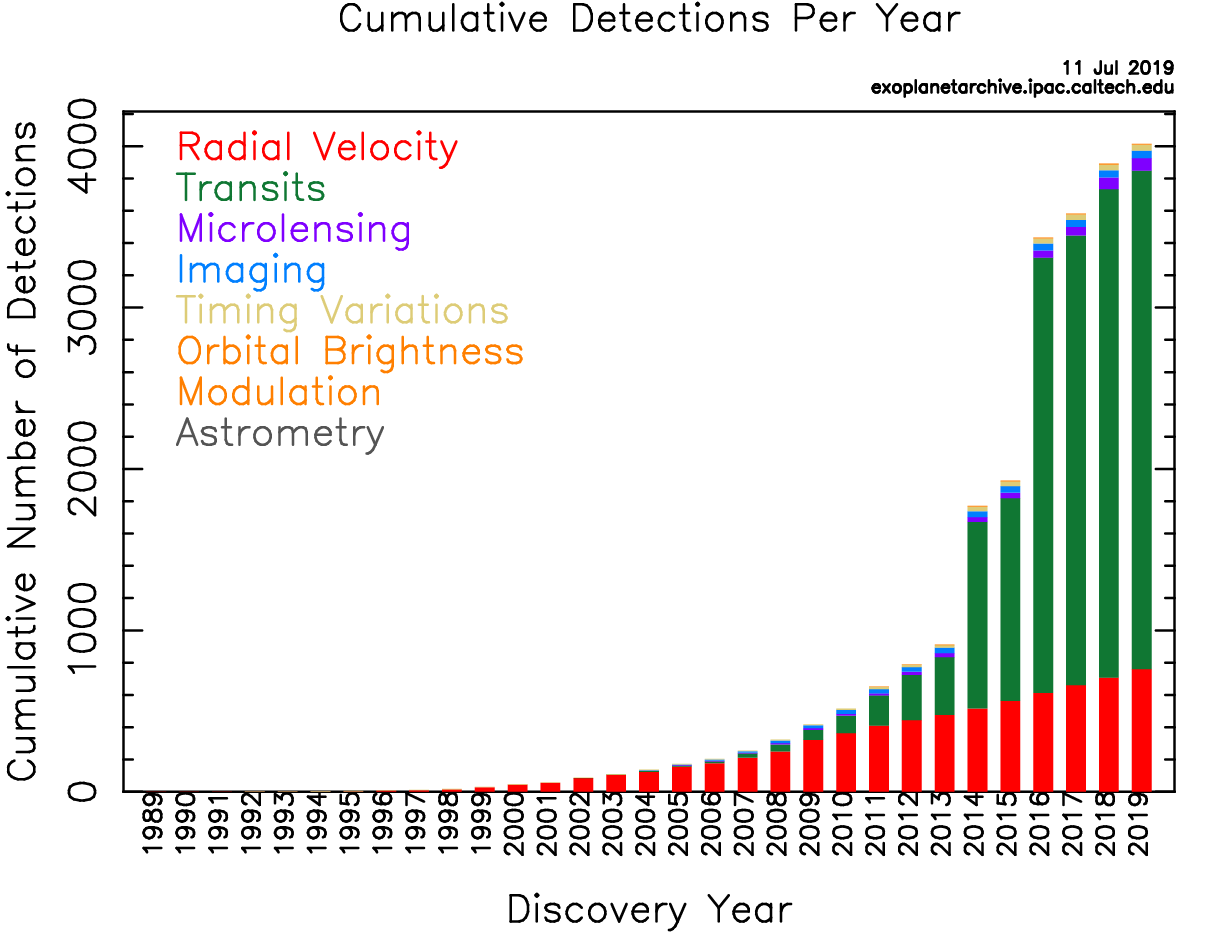
\includegraphics[width=0.7\columnwidth]{imagenes/exo_dischist_cumulative.png}
\caption{Accumulative number of discovered exoplanets by year.}
\label{amount_exoplanet}
\end{figure}

The light curve produced by a transit event provides important information of the planetary system. For example, it is the only way on which we can derived directly the proportion between the exoplanet and star radius. It can also give information about the impact parameter, and therefore, the inclination of the orbit. 

In Figure~\ref{transit} is described the architecture of a transiting exoplanet. Thanks to its geometry, the transit event as well as some parameters of the planetary system can be described with a few simple relations (cite Seager and Mallean y Winn).  When the planet passes in front of its star produced a dimming in its flux called primary transit. The maximum drop during the transit event defines the transit depth $\Delta{F}$:

\begin{equation}
    \Delta{F} = \left(\frac{R_{p}}{R_{*}}\right)^2 
\end{equation}

Where $R_{p}$ and $R_{*}$ are the planet and star radius, respectively. The numbers 1, 2, 3 and 4 correspond to the contact times: $t_{1}$, $t_{2}$, $t_{3}$ and $t_{4}$. The total duration of the transit is $t_{T} = t_{4}-t_{1}$ and the full duration is $t_{F}=t_{3}-t_{2}$. The total duration of the transit can be also described considering planetary parameters such as the period $P$, semi-major axis $a$ and orbital inclination $i$:

\begin{equation}
    t_{T} = \frac{PR_{*}}{\pi a} \sqrt{\left(1+\frac{R_{p}}{R_{*}}\right)^2-\left(\frac{a\cos i}{R_{*}}\right)}
\end{equation}

The impact parameter $b$, is the sky-projected distance between the center of the star and the planet at conjunction:

\begin{equation}
    b = \frac{a\cos{i}}{R_{*}}\left(\frac{1-e^2}{1+e\sin{\omega}}\right)
\label{impact_param}
\end{equation}

Where $\omega$ is the periastron longitude. In the case of circular orbits, the eccentricity is zero, thus Eq.~\ref{impact_param} is simplified to:

\begin{equation}
    b = \frac{a\cos{i}}{R_{*}}
\label{impact_param_simple}
\end{equation}

\begin{figure}[H]
\centering
\includegraphics[width=1.0\columnwidth]{imagenes/transit_architecture.pdf}
\caption{Architecture of a transiting exoplanet and the observed light curve. Based on the light curve itself it is possible to measure the transit depth $\Delta F$, the impact parameter $b$. From them, the planet-to-star radius ratio $R_{p}/R_{*}$ and the orbital inclination $i$ can be derived. Figure from The Handbook of Exoplanets by M. Perryman.}
\label{transit}
\end{figure}

Depending on the orbital and physical parameters of the exoplanet, the shape of the observed light curve will vary. For example, Figure \ref{transit_examples} shows how the light curve reflects the configuration of the system. Hot Jupiters are the kind of planet easier to detect, since their planet-to-star radius ratio is larger. But an smaller planet orbiting a dwarf star could produce a similar ratio of the radius. In the other hand, exoplanets with larger orbital inclinations will produce shorter drops in the flux, in comparison with planets in the same orbital-plane with the host star.     

\begin{figure}[H]
\centering
\includegraphics[width=0.8\columnwidth]{imagenes/transit_example.pdf}
\caption{Examples of transiting exoplanets and how their light curves differ between them thanks to the physical properties of the exoplanet.}
\label{transit_examples}
\end{figure}

\section{Transit Timing Variations}

Since the discovery of the first exoplanet, one of the principal questions that arose was: are they alone in their systems? The idea of multiplanetary systems is a consequence of our knowledge about the planetary system where we live in, and until today the Solar System has the larger number of orbiting planets. Besides the Solar System, Kepler-90 has the same number of confirmed exoplanets: eight. Statistically, around a 20\% of the confirmed exoplanets live in a multiplanetary system, but this number is theoretically larger (cite). 

The Transit Timing Variations (TTV) technique was first proposed as a way to detect Earth-mass planets in multiplanetary systems due to gravitational interactions with a transiting exoplanet \citep{Holman2005,Agol2005}. However, TTVs can be also use to measure tidal interactions between the planet and the star or to detect exomoons \citep{Kipping2009a,Kipping2009b}, among others. 

For a given light curve of a transiting exoplanet (see Fig. \ref{transit}), the transit time $T_{c}$ (or central time of the transit) is computed as:

\begin{equation}
T_{c} = \frac{t_T}{2}
\end{equation}

A single transiting planet will stay in a Keplerian orbit around its host star, producing a transit time strictly periodic. Thus, the transit time $T_c$ follows a linear function of the orbital period $P$: 

\begin{equation}
T_{c}(E) = T_{0} + E \cdot P
\label{linear_ephemeris} 
\end{equation}

Where $T_0$ is a reference transit time and $E$ is the number of epochs since $T_0$.  The presence of a second planet produces transits no exactly periodic, hence Eq.~\ref{linear_ephemeris} will not be valid. As the transit times will be no longer a linear function,  the time between  transits varies.  The variation in time produced by the perturbing body depends on the mass and geometry of their orbits. The magnitude of this variation between successive transits of the transiting planet is:

\begin{equation}
\Delta t = \frac{45\pi}{16} \frac{M_2}{M_*} P_{1} \alpha^3_{e} (1-	\sqrt{2}\alpha^{3/2})^{-2}
\label{delta_t}
\end{equation}

Where $\alpha_e = a_1/(a_2(1-e_2))$ is the ratio of the semi-major axis of the planets, considering a nonzero eccentricity for the perturbing planet ($e_2 \neq 0$) and $a_1 < a_2$. The semi-major axis of the transiting exoplanet is $a_1$ and its orbital period $P_1$, while the perturbing planet has a mass $M_2$, semi-major axis $a_2$, orbital period $P_2$ and eccentricity $e_2$. Assuming that the orbital parameters of the known transiting exoplanet are already derived from its light curve, the orbital parameters and mass of the hypothetical pertuber can be estimate numerically \citep{Nesvorny2008,Nesvorny2009}, even if the second planet does not transit the star. 

The TTV method is a efficient tool to search for additional unseen companions, since in order to employ this technique only photometry of the transiting exoplanet during a transit events is required. Moreover, this technique enhances its sensitivity when the two bodies in the system are close to Mean Motion Resonances (MMR) \citep{Agol2005,Steffen2005,Agol2007} (see Figure~\ref{rms_ttv_amplitude}) . 

\begin{figure}
\centering
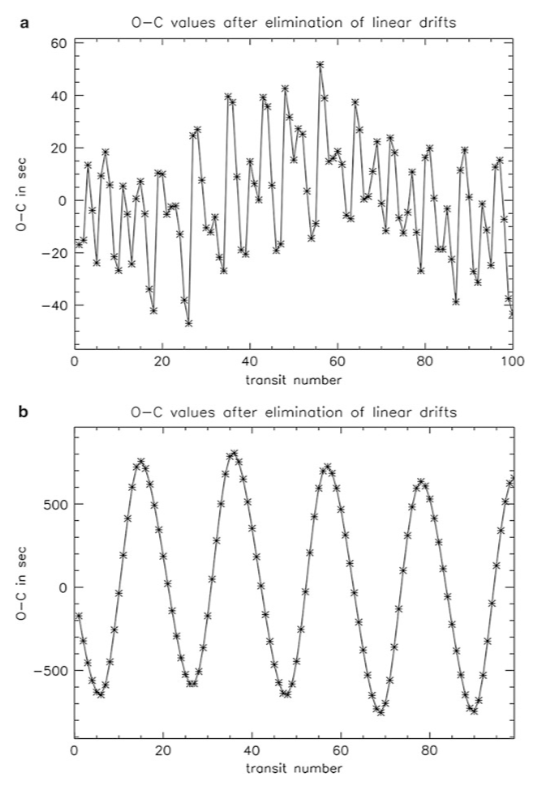
\includegraphics[width=0.6\columnwidth]{imagenes/rms_ttv_amplitude}
\caption{Example of a system with a transiting exoplanet of $1~M_{J}$ in a 10-day orbit, around a star with $0.367~M_{\odot}$. The perturber is a Earth-mass planet. Panel \textbf{a} is an O-C diagram showing the measured TTV when the pertuber has a period of 16.11 days, not in Mean Motion Resonance with the transiting planet. Panel \textbf{b} shows the TTV when the transiting planet and the perturbing planet are near an interior 2:1 resonance. The amplification of the TTV signal is by an order of magnitude. (Figure from \cite{Haghighipour2011})}
\label{rms_ttv_amplitude}
\end{figure}

\cite{Holman2010} presented the first multiplanetary system confirmed using the TTV method: Kepler-9b and Kepler-9c. This two Saturn-size planets are in near 2:1 orbital resonance with periods of 19.2 and 38.9 days.

The no detection of TTV is also important: architecture of the system.


